\chapter{Dataset\label{chap:dataset}}

One of the most important step of a machine learning design methodology is the collection of dataset that represents the problem we wish to solve. We used two popular and published network capture dataset that contains malware and benign traffic.

\begin{itemize}
	\item CTU-13 Dataset \cite{GarciaGSZ14}
	
	The CTU-13 dataset was captured in the Czech Technical University, Czech Republic. It is a set of 13 different malware traffic captures which includes normal, malware and background traffic. Each malware traffic was captured by executing the malware in a Windows virtual machine and recording the network traffic on that host. The normal traffic corresponds to network traffic which was captured on normal hosts, i.e. hosts which weren't infected with malware. We will only be using only normal and malware traffic which are stored in pcap files. 
	
	\item Malware Capture Facility Project \cite{Erquiaga15}
	
	This research project is also carried out at Czech Technical University ATG Group to capture, analyze and publish long-lived real malware network traffic. The dataset was contributed by Maria Jose Erquiaga. The malware was executed with two restrictions: a bandwidth limit and spam interception. The most important characteristic of this project is the execution of malware during long periods of time, that can go up to several months. The traffic is stored in pcap files, labeled and made public for the research community
	
\end{itemize}

The entire dataset consists of total 72 captures out which 59 are malware captures and 13 are benign captures. Table \ref{tab:1} gives us basic statistics about our dataset.

\begin{table}[!htb]
	\caption{Dataset Statistics\label{tab:1}}
	\begin{center}
		\begin{tabular}{p{0.43\textwidth}|c}\hline\hline
			Total Number of connection 4-tuples & 61726 \\
			Number of normal 4-tuples & 8828 \\
			Number of malware 4-tuples & 52898 \\
			Total number of flows & 1136631\\
			Normal flows & 69358\\
			Malware flows & 1067273\\
			\hline\hline
		\end{tabular}
	\end{center}
\end{table}

\section{Data Structure}

Each dataset contains a pcap file of the capture, list of infected and normal hosts and Bro IDS logs generated using the pcap files. Bro \cite{Bro} is a powerful open-source network analysis and intrusion detection tool. It supports various network analysis features traffic inspection, log recording, attack detection, etc. We use Bro to generate various network traffic logs which describe the network flow information and other metadata. This information is then used to extract various features about the traffic flow and use the those features to train and test machine learning models. Bro generates various log files but we are mainly interested on the following three log files:

\begin{enumerate}
	\item conn.log : It contains information about TCP, UDP and ICMP connections.
	\item ssl.log: It contains information about SSL/TLS certificates and sessions.
	\item x509.log: It contains information about X.509 certificates.
\end{enumerate}

\section{Feature Extraction}

We extracted several features from the Bro logs generated using the network captures. Features related to a single connection is spread over different log files. For example, if we have an SSL connection to some server, the connection features such as source, destination IP addresses, ports, protocols, connection duration, etc. are stored in connection log (conn.log). The SSL features such as cipher used,  server name, etc. are stored in SSL log (ssl.log) and certificate features such as key lengths, common names, validities, subjects, etc. are stored in certificate logs (x509.log). Bro provides interconnection between various logs using unique keys. These unique keys are common for a connection across different logs provided by Bro as shown in Figure \ref{fig:interconnection}. Hence, an SSL connection will have the same unique key to identify the record in connection and SSL logs. SSL has certificate ids to uniquely identify x509 certificates in certificate logs which were used in the SSL session or connection.

\begin{figure}[htb]
	\begin{center}
		\begin{subfigure}{1\textwidth}
			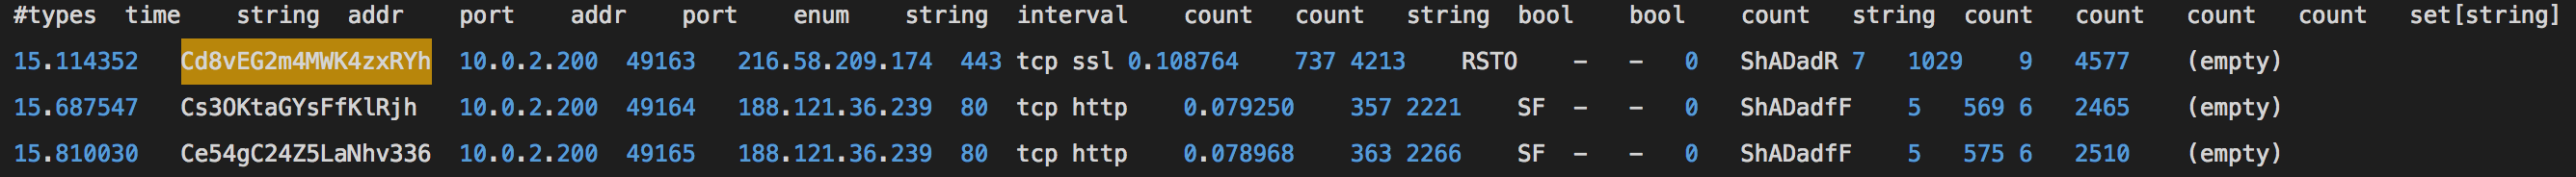
\includegraphics[width=1\textwidth]{images/conn-log.png} 
			\caption{conn.log}
			
			\vspace{0.4cm}
			
		\end{subfigure}
		\begin{subfigure}{1\textwidth}
			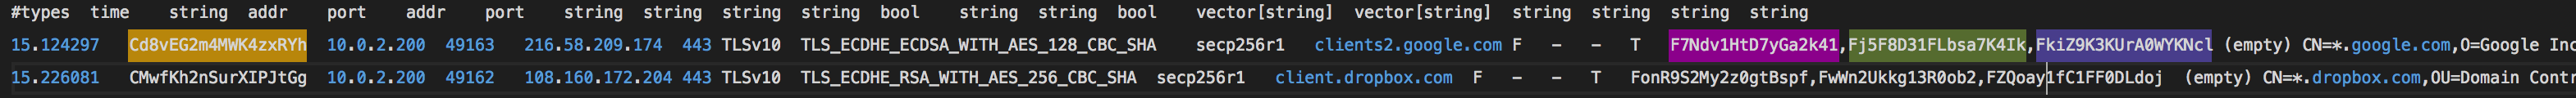
\includegraphics[width=1\textwidth]{images/ssl-log.png} 
			\caption{ssl.log}
			
			\vspace{0.4cm}
			
		\end{subfigure}
		\begin{subfigure}{1\textwidth}
			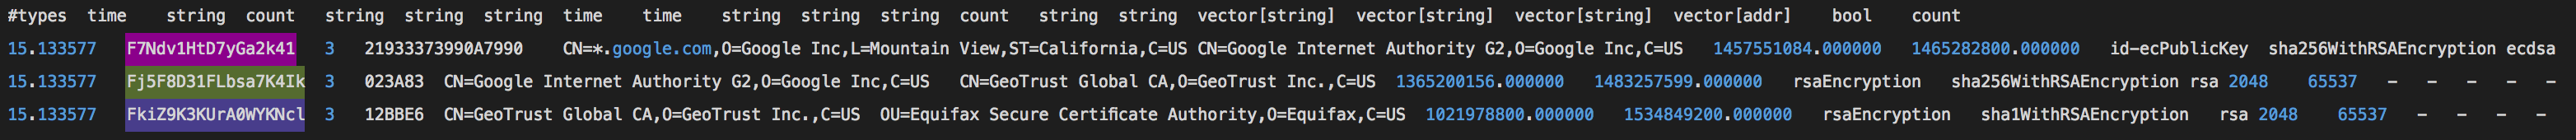
\includegraphics[width=1\textwidth]{images/x509-log.png}
			\caption{x509.log}
		\end{subfigure}
	\end{center}
	\caption{Interconnection of log records using unique keys in Bro} 
	\label{fig:interconnection}
\end{figure}

Bro tracks every incoming and outgoing connection in conn.log. Every record in the conn.log gives us information about a particular connection. Since we are interested only in encrypted network connection, i.e. HTTPS, we only consider connection records that are related to HTTPS connections. Since HTTPS connection uses SSL/TLS to protocols to establish an encrypted link between the client and the server, we only extract connection records which have corresponding entries in the ssl.log file. This can be achieved by going through all the records in ssl.log file and extracting corresponding connection records from the conn.log file.

Since, every SSL/TLS connection requires a server certificate to ensure credibility of the server \cite{RFC1601}, every record in ssl.log contains one or more than one unique certificate ids that the server offered to validate its signing chain. The unique certificate ids represent the certificate record in the x509.log file. We extract only the first certificate id from the ssl.log file since the it corresponds to the end-user certificate. The remaining ids correspond to intermediate and root certificates.

Every connection record can be identified by the 4-tuple of source IP address, destination IP address, destination port and protocol. We use this 4-tuple as key to aggregate network features. Hence every connection which has the same 4-tuple key is grouped together. We then extract features from each group of connection records which were aggregated in the previous step.

\section{Features}

We extracted some features based on \cite{Frantisek2017, AndersonM16} from the connection, SSL and certificate log files from Bro. Table \ref{tab:1} contains connection features extracted from conn.log, Table \ref{tab:2} contains SSL features extracted from ssl.log and Table \ref{tab:3} contains certificate features extracted from x509.log. All the features are computed over a single connection 4-tuple aggregate of records.

\begin{table}[!htb]
	\caption{Extracted Features from conn.log\label{tab:2}}
	\begin{center}
		\begin{tabular}{c|p{0.40\textwidth}|p{0.50\textwidth}}\hline\hline
			S.No & Feature Name & \multicolumn{1}{l}{Description} \\ \hline
			1 & no\_of\_flows & Number of aggregated records in connection 4-tuple\\
			2 & avg\_of\_duration & Mean duration of connections \\
			3 & standard\_deviation\_of\_duration & Standard deviation of connections\\
			4 & percent\_sd\_of\_duration & Percentage of records with duration greater than standard deviation\\
			5 & size\_of\_orig\_flows & No. of bytes sent by the originator\\
			6 & size\_of\_resp\_flows & No. of bytes sent by the responder\\
			7 & ratio\_of\_sizes & Ratio of responder bytes by all bytes transmitted \\
			8 & percent\_of\_established\_conn & Percentage of established connections out of all attempted connections\\
			9 & inbound\_pckts & No. of incoming packets\\
			10 & outbound\_pckts & No. of outgoing packets\\
			11 & periodicity\_average & Mean of periodicity of connection\\
			12 & periodicity\_standart\_deviation & Standard deviation of periodicity of connection\\
			\hline\hline
		\end{tabular}
	\end{center}
\end{table}

\begin{table}[!htb]
	\caption{Extracted Features from ssl.log\label{tab:3}}
	\begin{center}
		\begin{tabular}{c|p{0.35\textwidth}|p{0.50\textwidth}}\hline\hline
			S.No & Feature Name & \multicolumn{1}{l}{Description} \\ \hline
			1 & ssl\_ratio & Ratio of SSL records to non-SSL records\\
			2 & tls\_version\_ratio & Ratio of records with TLS \\
			3 & SNI\_ssl\_ratio & Ratio of connections having Server Name Indication (SNI) in SSL record\\
			4 & self\_signed\_ratio & Ration of connection with self signed certificates\\
			5 & SNI\_equal\_DstIP & 1 if SNI is equal to destination IP in SSL record\\
			6 & differ\_SNI\_in\_ssl\_log & Ratio of SSL records with different SNI\\
			7 & differ\_subject\_in\_ssl\_log & Ratio of SSL records with different subjects than certificate\\
			8 & differ\_issuer\_in\_ssl\_log & Ratio of SSL records with different issuer than certificate\\
			9 & ratio\_of\_same\_subjects & Ratio of SSL records with same subject as certificate\\
			10 & ratio\_of\_same\_issuer & Ratio of SSL records with same issuer as certificate\\
			11 & is\_SNI\_top\_level\_domain & 1 if SNI is a top level domain\\
			12 & ratio\_missing\_cert & Ratio of records with missing certificates\\
			\hline\hline
		\end{tabular}
	\end{center}
\end{table}

\begin{table}[!htb]
	\caption{Extracted Features from x509.log\label{tab:4}}
	\begin{center}
		\begin{tabular}{c|p{0.35\textwidth}|p{0.50\textwidth}}\hline\hline
			S.No & Feature Name & \multicolumn{1}{l}{Description} \\ \hline
			1 & avg\_key\_len & Average cipher key length\\
			2 & avg\_of\_certificate\_len & Average certificate length\\
			3 & standart\_deviation\_cert\_len & Standard deviation of certificate length\\
			4 & is\_valid\_certificate & 1 if the certificate is valid during capture\\
			5 & amount\_diff\_certificates & No. of different certificates\\
			6 & no\_of\_domains\_in\_cert & No. of domains in certificates\\
			7 & certificate\_ratio & Ratio of certificates validity time lengths\\
			8 & no\_of\_cert\_path & No. of signed certificates paths\\
			9 & x509\_ssl\_ratio & Ratio of SSL logs with x509 certificates\\
			10 & is\_SNIs\_in\_SAN\_dns & Checks if SNI is SAN DNS\\
			11 & is\_CNs\_in\_SAN\_dns & 1 if all certificates have Comman Names in SAN\\
			12 & differ\_subject\_in\_cert & Ratio of different subject in certificates\\
			13 & differ\_issuer\_in\_cert & Ratio of different issuer in certificates\\
			14 & differ\_sandns\_in\_cert & Ratio of different SAN DNS in certificates\\
			15 & is\_same\_CN\_and\_SNI & Checks if CN is same as SNI\\
			16 & average\_certificate\_expo & Average of certificate exponent\\
			17 & ratio\_certificate\_path\_error & Checks if certificate path is valid\\
			\hline\hline
		\end{tabular}
	\end{center}
\end{table}

\section{Labels}

The dataset from \cite{GarciaGSZ14} and \cite{Erquiaga15} contains IP addresses of infected and normal hosts. We use these IP addresses to label our dataset accordingly. Hence, if a connection record has an infected IP address either as source or destination then the record is classified as malware else it is classified as benign. 